\documentclass[11pt]{article}
% =====================================================================
%  NGRAM-pro family --- the one program-feature category, explained,
%  plus the two honest inconclusives that bound it.
%  Companion to i2s_pro_categories.tex / vp_pro_categories.tex.
%  Every cited branch + value is REAL (bench/dataset.jsonl +
%  step5b_new_v3/ngram_coverage_WL/{evidence_test,assignments_sB}.json +
%  the per-branch cards/analyses). All four branches are libxml2, whose
%  corpora + source live on server sB and are verified there.
%  Compile: pdflatex ngram_pro_categories.tex  (needs tikz + pgfplots + listings)
% =====================================================================
\usepackage[margin=1in]{geometry}
\usepackage{amsmath,amssymb}
\usepackage{xcolor}
\usepackage{listings}
\usepackage{booktabs}
\usepackage{tikz}
\usepackage{pgfplots}
\pgfplotsset{compat=1.16}
\usetikzlibrary{arrows.meta,positioning,shapes.geometric}

\definecolor{winc}{RGB}{30,120,60}   % winner (naive_ngram4 resolves) green
\definecolor{losc}{RGB}{190,60,60}   % loser  (plain naive blocks)    red
\definecolor{codebg}{RGB}{246,246,248}
\definecolor{kw}{RGB}{40,60,150}
\definecolor{cmt}{RGB}{120,120,120}
\definecolor{str}{RGB}{160,60,20}

\lstdefinestyle{c}{
  language=C, basicstyle=\ttfamily\small, backgroundcolor=\color{codebg},
  keywordstyle=\color{kw}\bfseries, commentstyle=\color{cmt}\itshape,
  stringstyle=\color{str}, numbers=none, frame=single, framerule=0pt,
  framesep=6pt, breaklines=true, showstringspaces=false, xleftmargin=4pt,
}

% A small "metric & rule" box used under every category.
\newcommand{\metricbox}[4]{%
  % #1 tool  #2 metric (plain meaning)  #3 verify rule  #4 real example
  \par\smallskip\noindent\fbox{\parbox{\dimexpr\linewidth-2\fboxsep-2\fboxrule}{%
  \footnotesize
  \textbf{Tool:}~\texttt{#1}\\[2pt]
  \textbf{Metric:}~#2\\[2pt]
  \textbf{Verify rule (the arbiter fires this, no LLM):}~\texttt{#3}\\[2pt]
  \textbf{Real example:}~#4}}\par\smallskip}

\title{\textbf{The NGRAM-pro family: why path-context coverage reaches deeper}}
\author{}
\date{}

\begin{document}
\maketitle
\vspace{-3em}

\paragraph{Backdrop.} \emph{NGRAM-pro} collects the roadblocks where a fuzzer that
keys coverage on \emph{the last few edges it walked} (\texttt{naive\_ngram4}'s
$4$-edge path-tuple feedback) gets through, while plain single-edge coverage
(\texttt{naive}) stays stuck. The mechanism is not about \emph{values} at all ---
unlike I2S (paste the right bytes) or VP (climb a per-byte gradient), n-gram
coverage changes \emph{what counts as new}. It folds the last four edge IDs into
the map key, so the \emph{same} basic block, reached through a different
$4$-edge path, lands in a \emph{fresh} bucket and the seed that produced it is
retained. Picture a maze where plain coverage only remembers ``I've stood on this
tile'' --- so it throws away the seed the second time it reaches a junction by a
longer route --- while n-gram remembers ``I've stood on this tile \emph{having
come from there, via there, via there}''. That extra memory keeps the
intermediate seeds that march a sequential decoder one step \emph{deeper} each
time; plain coverage collapses them to an already-seen edge and discards them, so
its corpus never accumulates the depth the gate needs. Counts are validated
roadblocks ($n$); a branch joins NGRAM-pro by its \emph{deciding pair}
(\texttt{naive\_ngram4} resolves, plain \texttt{naive} blocks), not by the raw
4-char shape. The family is small and \emph{honest} about it: one discriminable
category, and two branches we leave \texttt{inconclusive} on principle (\S2)
because no built measurement can separate path-retention from plain luck there.

% =====================================================================
\section*{1.\ \ The path memory reaches a deeper decode state \hfill {\footnotesize\texttt{ngram\_sequential\_depth\_reach} ($n=2$)}}
The whole validated family. The gate sits at the bottom of a \emph{sequential}
decode --- a loop that consumes one code unit / one digit / one dispatch step at a
time, with its own edge each pass. Each iteration through that region produces a
new $4$-edge path tuple, so \texttt{naive\_ngram4} keeps the seed that got one
step further in; plain \texttt{naive} sees the same block again, calls it
``covered'', and drops the seed. Over the campaign the n-gram corpus drifts toward
inputs that drive the decoder \emph{deep enough to reach the gate}; the
single-edge corpus stalls shallow. The tell is not ``the right bytes are present''
--- it is ``the n-gram seeds execute the blocker line far more / drive it much
further in.''

\begin{lstlisting}[style=c]
// libxml2  encoding.c : UTF16LEToUTF8()   -- assemble a UTF-16 surrogate pair
while (in < inend) {
    c = *in++; c |= (*in++) << 8;          // little-endian 16-bit code unit
    if ((c & 0xFC00) == 0xD800) {          // <-- blocker (libxml2/6325): high surrogate
        d = *in++; d |= (*in++) << 8;      //     lines 534-545: only the winner gets here
        c = ((c & 0x3FF) << 10) + (d & 0x3FF) + 0x10000;
    }
    /* ... emit UTF-8 ... */               // each pass is a fresh 4-edge path tuple
}
\end{lstlisting}

\noindent\textbf{How we know it is really the path memory.} We replay each side's
seed set through the instrumented binary and count, per seed, how many times the
blocker line executes (its sequential-decode \emph{depth}) and whether the seed
takes the decisive side. The \texttt{naive\_ngram4} arm should reach the line far
more. Crucially this \emph{discriminates}: a plain literal-failure story (``naive
just lacks the right bytes'') predicts the loser reaching the \emph{same} depth and
failing the final compare ($\texttt{depth\_lift}\approx1$); n-gram retention
predicts the loser stalled \emph{shallow}, never arriving.

\metricbox{depth\_reach}
{\texttt{depth\_lift} = winner / loser per-seed executions of the blocker line;
\texttt{side\_lift} = how much more the winner takes the decisive branch;
\texttt{winner\_deeper} (bool)}
{depth\_lift >= 1.5 AND winner\_depth > loser\_depth}
{libxml2/6325 (\texttt{UTF16LEToUTF8}, the high-surrogate gate \texttt{(c \& 0xFC00) == 0xD800}, \texttt{encoding.c:533}) --- \texttt{winner\_depth}$=156.7$ vs \texttt{loser\_depth}$=95.5$, so \texttt{depth\_lift}$=1.64$ and \texttt{side\_lift}$=1.55$: the n-gram corpus drives the UTF-16 decode loop ${\approx}1.6\times$ deeper per seed and into the surrogate-assembly lines 534--545 that the plain-\texttt{naive} corpus never reaches.}

\begin{center}
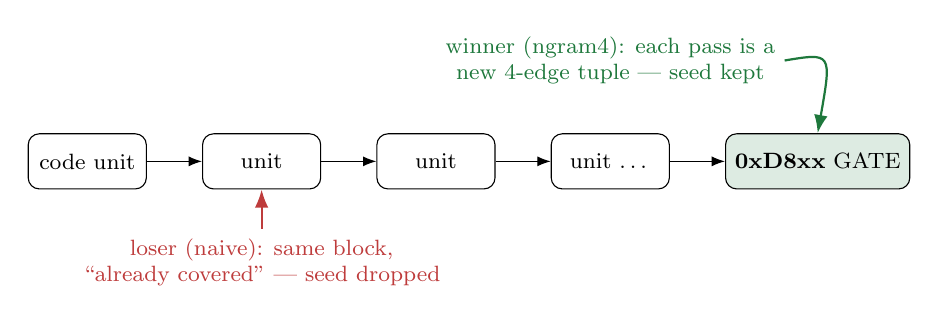
\begin{tikzpicture}[font=\footnotesize,>=Latex,node distance=7mm]
\tikzstyle{f}=[draw,rounded corners,minimum width=15mm,minimum height=7mm]
\node[f] (a) {code unit};
\node[f,right=of a] (b) {unit};
\node[f,right=of b] (c) {unit};
\node[f,right=of c] (d) {unit \dots};
\node[f,right=of d,fill=winc!15] (e) {\textbf{0xD8xx} GATE};
\draw[->] (a)--(b); \draw[->] (b)--(c); \draw[->] (c)--(d); \draw[->] (d)--(e);
% loser stalls shallow
\node[losc,below=5mm of b,align=center] (l) {loser (naive): same block,\\``already covered'' --- seed dropped};
\draw[->,losc,thick] (l) -- (b.south);
% winner reaches gate
\node[winc,above=5mm of d,align=center] (w) {winner (ngram4): each pass is a\\new 4-edge tuple --- seed kept};
\draw[->,winc,thick] (w.east) .. controls +(0.6,0.1) .. (e.north);
\end{tikzpicture}\\[2pt]
{\footnotesize Plain coverage forgets the path, so it discards the seed that reached
the junction by a longer route; the n-gram key remembers the route, keeps the seed,
and the corpus walks one step deeper each generation until it reaches the gate.}
\end{center}

\paragraph{Second member: a content-dispatch fan.} The same memory, a different
shape of ``deeper.'' Here the gate is the \texttt{'<![CDATA['} opener test
(\texttt{cur[6] == 'T'}); the \emph{winner} takes its \emph{false} side and pours
into the sibling content branches --- end-tag \texttt{'</'}, PI \texttt{'<?'},
start-tag, char-data --- each its own $4$-edge tuple. The n-gram corpus keeps that
\emph{diversity} of non-CDATA seeds; plain coverage gives no extra credit for the
path context, so those seeds are under-retained and short CDATA fragments dominate
the loser's corpus instead.

\metricbox{depth\_reach}
{same tool, second branch --- per-seed executions of the dispatch blocker line}
{depth\_lift >= 1.5 AND winner\_depth > loser\_depth}
{libxml2/6835 (\texttt{xmlParseTryOrFinish}, the \texttt{'<![CDATA['} dispatch at \texttt{parser.c:11752}, operand \texttt{'T'}) --- \texttt{winner\_depth}$=45.1$ vs \texttt{loser\_depth}$=15.2$, \texttt{depth\_lift}$=2.97$: the n-gram corpus reaches the content-dispatch chain ${\approx}3\times$ more per seed. (\texttt{side\_lift}$=0.9$ here because the winner takes the dispatch \emph{false} side --- it is reaching the region more often, not crossing the same edge.)}

\begin{center}
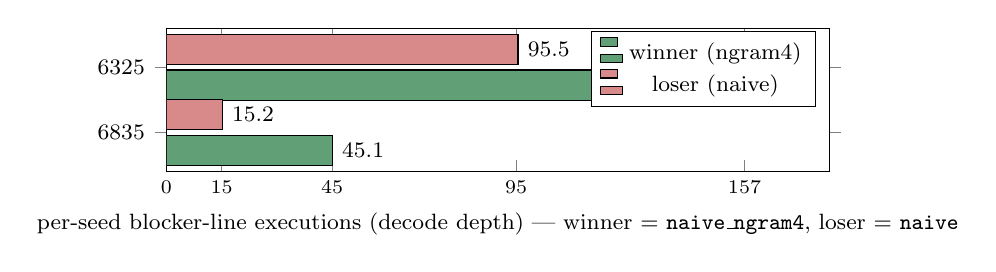
\begin{tikzpicture}
\begin{axis}[
  width=10cm, height=3.4cm, xbar, xmin=0, xmax=180,
  bar width=11pt, enlarge y limits=0.6,
  symbolic y coords={6835, 6325},
  ytick=data, yticklabel style={font=\footnotesize}, xtick={0,15,45,95,157},
  xticklabel style={font=\scriptsize},
  nodes near coords, every node near coord/.append style={font=\footnotesize},
  xlabel={\footnotesize per-seed blocker-line executions (decode depth) --- winner = \texttt{naive\_ngram4}, loser = \texttt{naive}},
]
\addplot[fill=winc!70] coordinates {(156.7,6325) (45.1,6835)};
\addplot[fill=losc!60] coordinates {(95.5,6325) (15.2,6835)};
\legend{\footnotesize winner (ngram4), \footnotesize loser (naive)}
\end{axis}
\end{tikzpicture}\\[-1pt]
{\footnotesize Both validated branches: the n-gram corpus drives the sequential
blocker far deeper per seed ($\texttt{depth\_lift}=1.64$ and $2.97$), clearing the
$\ge1.5$ bar; the single-edge corpus stalls shallow.}
\end{center}

% =====================================================================
\section*{2.\ \ Where we stop: two honest inconclusives}
NGRAM-pro is deliberately the smallest \emph{pro} family, and the reason is a
property of the technique, not a gap in the data. n-gram coverage is a
\emph{non-local} feedback --- its effect lives in \emph{path tuples across the
whole campaign}, not in any one branch's bytes --- so once a gate offers neither a
\emph{depth} gradient nor a \emph{value} gradient, no branch-local measurement we
have can separate ``path-retention got us here'' from ``a luckier corpus got us
here.'' Per the project's G3 guardrail (keep honest \texttt{inconclusive}s; don't
chase 100\%), we label these two and stop rather than force a story.

\begin{center}\small
\begin{tabular}{@{}llp{8.4cm}@{}}
\toprule
\textbf{branch} & \textbf{gate} & \textbf{why no built tool discriminates} \\
\midrule
libxml2/6359 & \texttt{0xEFBBBF} UTF-8 BOM &
\emph{Flat} 3-byte equality cascade (\texttt{in[0]==0xEF \&\& in[1]==0xBB \&\& in[2]==0xBF}): no decode loop, so \texttt{depth\_reach} is \emph{undefined} (no stage to climb). A Hamming-distance test \emph{could} run, but a winner corpus closer to the BOM triple is equally consistent with plain literal-presence as with path-retention --- not discriminating (fails G1). \\
libxml2/6887 & \texttt{val < 0x800} overlong UTF-8 &
The loser \emph{reaches the comparison at the same depth} (\texttt{L T=0 F=1730}: it runs the 3-byte decode block $1730\times$), so \texttt{depth\_lift}$\approx1$ --- depth cannot separate the arms. \texttt{value\_distance\_reached} to the \texttt{0x800} threshold was applied and \emph{did not hold} (both arms sit at comparable magnitude distance); a relaxed re-test is forbidden. \\
\bottomrule
\end{tabular}
\end{center}

\noindent In both cases a round-3 pivot over the remaining registry tools
(\texttt{operand\_enrichment}, \texttt{joint\_necessity}, corpus-size / token-count)
was rejected on principle: \texttt{operand\_enrichment} needs a \texttt{cmplog}
arm this \texttt{naive\_ngram4}-vs-\texttt{naive} shape does not have, and the
volume tools measure \emph{whole-corpus} structure that a globally larger n-gram
campaign would inflate anyway --- so neither isolates path-tuple retention at the
gate. The honest \texttt{inconclusive} is the correct outcome.

% =====================================================================
\section*{At a glance}
\begin{center}\small
\begin{tabular}{@{}p{3.8cm}clp{4.8cm}@{}}
\toprule
\textbf{Category} & \textbf{$n$} & \textbf{Tool / metric} & \textbf{One-line reason} \\
\midrule
sequential depth reach & 2 & depth\_reach / \texttt{depth\_lift}, \texttt{side\_lift} & the 4-edge path memory keeps seeds that march the decoder deeper, so the n-gram corpus reaches the gate \\
\midrule
\textbf{NGRAM-pro total (validated)} & \textbf{2} & & \\
\midrule
honest inconclusive $\dagger$ & 2 & --- (no discriminating tool) & flat BOM cascade (no depth gradient) / overlong inequality (equal depth, equal value-distance) \\
\bottomrule
\end{tabular}
\end{center}

\noindent\footnotesize $\dagger$ Not part of the validated total. n-gram coverage
is a \emph{non-local} edge-tuple feedback: when a gate offers neither a depth nor a
value gradient, no branch-local registry tool can separate path-tuple retention
from a luckier corpus, so the branch is left \texttt{inconclusive} by design (G3).

\medskip\noindent\footnotesize Counts and example metrics regenerated from
\texttt{bench/dataset.jsonl} and
\texttt{step5b\_new\_v3/ngram\_coverage\_WL/\{evidence\_test,assignments\_sB\}.json};
the verify rule is the deterministic arbiter rule (no LLM in the decision). All
four branches are libxml2; their corpora and source live on server sB and the
gates are verified against the local source dumps there. The common thread is
\emph{path memory}: \texttt{naive\_ngram4} treats a block reached by a longer route
as new coverage, so it retains the intermediate seeds that walk a sequential
decoder deep enough to reach the gate --- depth the single-edge corpus collapses
and forgets.
\end{document}
